\documentclass{aip-cp}

\usepackage[numbers]{natbib}
\usepackage{rotating}
\usepackage{graphicx}
\usepackage{url}
\usepackage[utf8]{inputenc}

\begin{document}

\title{gamma-sky.net: Portal to the Gamma-Ray Sky}
\corresp[cor1]{Corresponding author: arjun.voruganti@gmail.com}

\author[mpik]{Arjun Voruganti\corref{cor1}}
\author[mpik]{Christoph Deil}
\author[mpik]{Axel Donath}
\author[mpik]{Johannes King}

\affil[mpik]{MPIK, Heidelberg, Germany}


\maketitle

\begin{abstract}
gamma-sky.net is a novel interactive website designed for exploring the gamma-ray sky, targeting both practitioners of astronomy and the general public alike. Our poster displays the content of our online portal, featuring high-energy survey images and catalog information using data from the Fermi Large Area Telescope (Fermi-LAT).  Users can interact with the archive through a pan-and-zoom feature and powerful search tools. As the field of gamma-ray astronomy develops, we plan on expanding the website with more publicly available gamma-ray data, including High Energy Spectroscopic System (H.E.S.S.) Galactic Plane Survey maps (upon their public release) and survey images from the Planck satellite. Along with enriching our database, we also aim to make available to the user additional engaging and resourceful tools, such as a display of spectral information. The website is being developed as an open-source, open-data project at \url{https://github.com/gammapy/gamma-sky}. Feedback and contributions are very welcome!

\end{abstract}

\section{References}

TODO: References that should be mentioned somewhere in the proceeding:

\begin{itemize}
    \item \cite{tevcat} -- TeVCat: An online catalog for Very High Energy Gamma-Ray Astronomy (\url{http://tevcat.uchicago.edu/})
    \item \cite{tgevcat} -- The Very High Energy source catalog at the ASI Science Data Center (\url{http://www.asdc.asi.it/tgevcat/})
    \item \cite{3fgl} -- Fermi Large Area Telescope Third Source Catalog 
    \item \cite{2fhl} -- 2FHL: The Second Catalog of Hard Fermi-LAT Sources
    \item \cite{snrcat} -- A census of high-energy observations of Galactic supernova remnants (\url{http://www.physics.umanitoba.ca/snr/SNRcat/})
    \item \cite{hips} -- Hierarchical progressive surveys (HIPS) (\url{http://aladin.u-strasbg.fr/hips/})
    \item \cite{aladin-lite} -- Aladin Lite: Embed your Sky in the Browser (\url{http://aladin.u-strasbg.fr/AladinLite/})
    \item \cite{gammapy} -- Gammapy - A Python package for gamma-ray astronomy (\url{http://gammapy.org/})
    \item 3FGL interactive table - (\url{http://fermi.gsfc.nasa.gov/ssc/data/access/lat/4yr_catalog/3FGL-table/})
    \item \cite{hgps} -- H.E.S.S. Galactic plane survey (HGPS) -- upcoming TeV maps and catalog we will add.
\end{itemize}


\section{Introduction}

The field of very-high-energy (VHE) astronomy is growing tremendously – while only a decade ago we observed no more than a handful of sources in the GeV range, today we have thousands, including hundreds within the TeV range. This advancement has been made possible due to our novel ground-based Cherenkov telescope instruments. Such systems exhibit more accurate source detections higher angular resolutions than ever before. Space-based satellites sharing similar technological breakthroughs have further developed the high-energy (HE) range of gamma-ray astronomy, as can be observed in the latest images from the Fermi Large Area Telescope (Fermi-LAT). As a whole, the instruments can capture gamma-rays in a wide spectrum of energies from 10 MeV to 10 TeV. The High Energy Stereoscopic System (H.E.S.S.) Galactic Plane Survey \cite{hgps}, the High-Altitude Water Cherenkov Observatory (HAWC) 1st Year Catalog, and the fourth Fermi-LAT Point Source Catalog (4FGL) are among the highly anticipated surveys that will be unveiled in the near future. Furthermore, with an incoming wave of notable systems planned to operate soon, such as the ground-based Cherenkov Telescope Array (CTA), we expect to discover numerous never-before-seen sources in the gamma-ray sky. With such abundance of HE and VHE sources and a rapid growth of interest in gamma-ray astronomy, there is an evident need for a central hub of all relevant catalog and image data. Our website (\url{http://gamma-sky.net}) was designed to function as such.

TODO: make sure these references are put in the appropriate places:

\begin{itemize}
    \item \cite{tevcat} -- TeVCat: An online catalog for Very High Energy Gamma-Ray Astronomy (\url{http://tevcat.uchicago.edu/})
    \item \cite{tgevcat} -- The Very High Energy source catalog at the ASI Science Data Center (\url{http://www.asdc.asi.it/tgevcat/})
    \item \cite{3fgl} -- Fermi Large Area Telescope Third Source Catalog
    \item \cite{2fhl} -- 2FHL: The Second Catalog of Hard Fermi-LAT Sources
    \item \cite{snrcat} -- A census of high-energy observations of Galactic supernova remnants (\url{http://www.physics.umanitoba.ca/snr/SNRcat/})
    \item \cite{hips} -- Hierarchical progressive surveys (HIPS) (\url{http://aladin.u-strasbg.fr/hips/})
    \item \cite{aladin-lite} -- Aladin Lite: Embed your Sky in the Browser (\url{http://aladin.u-strasbg.fr/AladinLite/})
    \item 3FGL interactive table - (\url{http://fermi.gsfc.nasa.gov/ssc/data/access/lat/4yr_catalog/3FGL-table/})
    \item \cite{hgps} -- H.E.S.S. Galactic plane survey (HGPS) -- upcoming TeV maps and catalog we will add.
\end{itemize}

\section{Idea}

\begin{itemize}

\item Interactive website designed for exploring the gamma-ray sky

\item Survey images of different frequency bands (mainly all-sky) overlaid onto a three-dimensional map. Gamma-ray sources from catalog data are pinpointed onto the map.

\item The website facilitates both quick browsing and deep investigation of sources

\item Understand the context of sources by viewing them on the map

\item Easily compare sources from different catalogs

\item Website targets professional astronomers, but also the general public through
a user-friendly interface and the easily understandable layout of sources plotted over a map.

\item Open source, open data - allows for 1. users to download any data from our website, and 2. for other developers to contribute to the code.

\end{itemize}


    gamma-sky.net is a one-stop resource for perusing images and catalogs but also closely examining a specific gamma-ray source.
    Although it was mainly built for the astronomical community, the webpage also targets the general public through a
    user-friendly interface and a clean information layout, all of which is compiled under cutting-edge web tools.

    Individuals who access the website via any modern internet browser will be welcomed with the Map View page.
    This page presents an overlay of multi-wavelength survey images, most of which are all-sky images, wrapped around a three-dimensional sphere.
    The map features pan-and-zoom functionality for easily navigating and quickly browsing the sky. Gamma-ray sources from
    our catalog data have been pinpointed onto the sphere, as shown in Figure~\ref{fig:mapview}. The map also utilizes a powerful search tool to either pan the view to a given sky position or locate a specific source by name. These features allow the user to easily find their sources and study their visual context in relation to other objects.
    gamma-sky.net additionally embodies a Catalog View, which incorporates more detailed information for each of the sources in our catalogs.
    Professional astronomers will navigate to this component of the website for the deep investigation of a particular source.
    See Figure~\ref{fig:catview} for the catalog view.

    It is imperative for all of our data on the online portal to be openly available for download and local analysis by any user. Additionally, gamma-sky.net is an open-source project and other developers are welcome to contribute to the code. We advise those interested in contributing to visit our Github repository at \url{https://github.com/gammapy/gamma-sky}.

\section{Features}

(Should we present this information in a bullet list or in paragraphs?)

\begin{enumerate}

\item Map View - easy navigation and quick browsing

  \begin{itemize}

  \item Pan and zoom the sky map by dragging and scrolling

  \item Toggle and view specific catalog layers and multi-wavelength survey images

  \item Pop-ups over each source for basic information

  \item Powerful search tools - locate objects by name, association, or coordinate position

  \item Export and share a specific view of the sky map via PNG

  \end{itemize}


\item Catalog View - deeply investigate a specific source

  \begin{itemize}

  \item Search tool to find a source in its respective catalog by source name

  \item Basic info, extension info, spectral info, distance info

  \item Light curves, emission spectra (currently only for 3FGL catalog)

  \item References to which telescope detected the source and links to where our data came from

  \end{itemize}


\item Further analysis of our data with tools like Gammapy (generate specific plots, etc.)

\item Mention again that all data is openly available for download

\end{enumerate}

\begin{figure}[h]
  \centerline{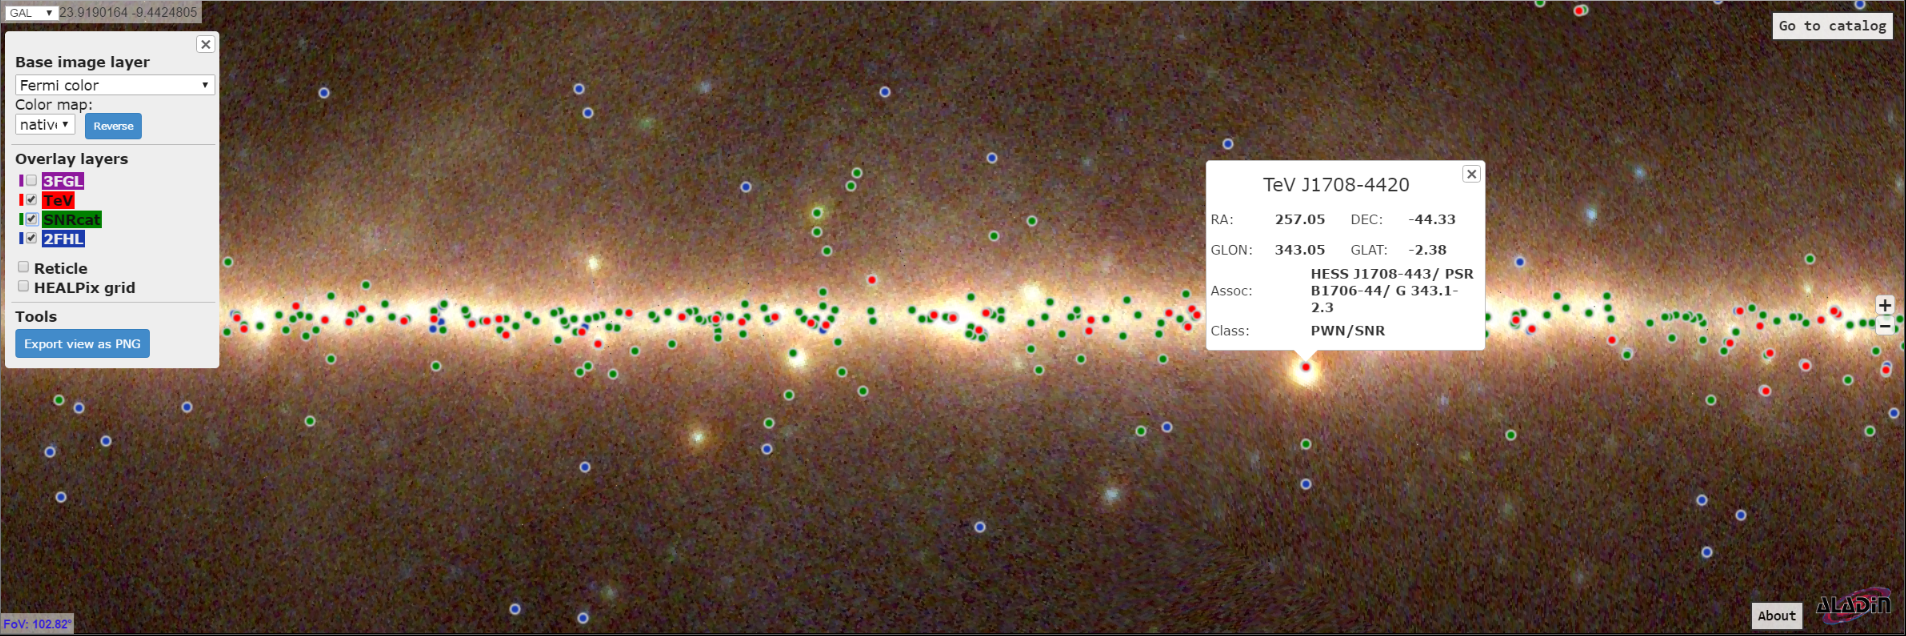
\includegraphics[width=\textwidth]{figures/mapview_wide}}
  \caption{Map View.}
\end{figure}

\begin{figure}[h]
  \centerline{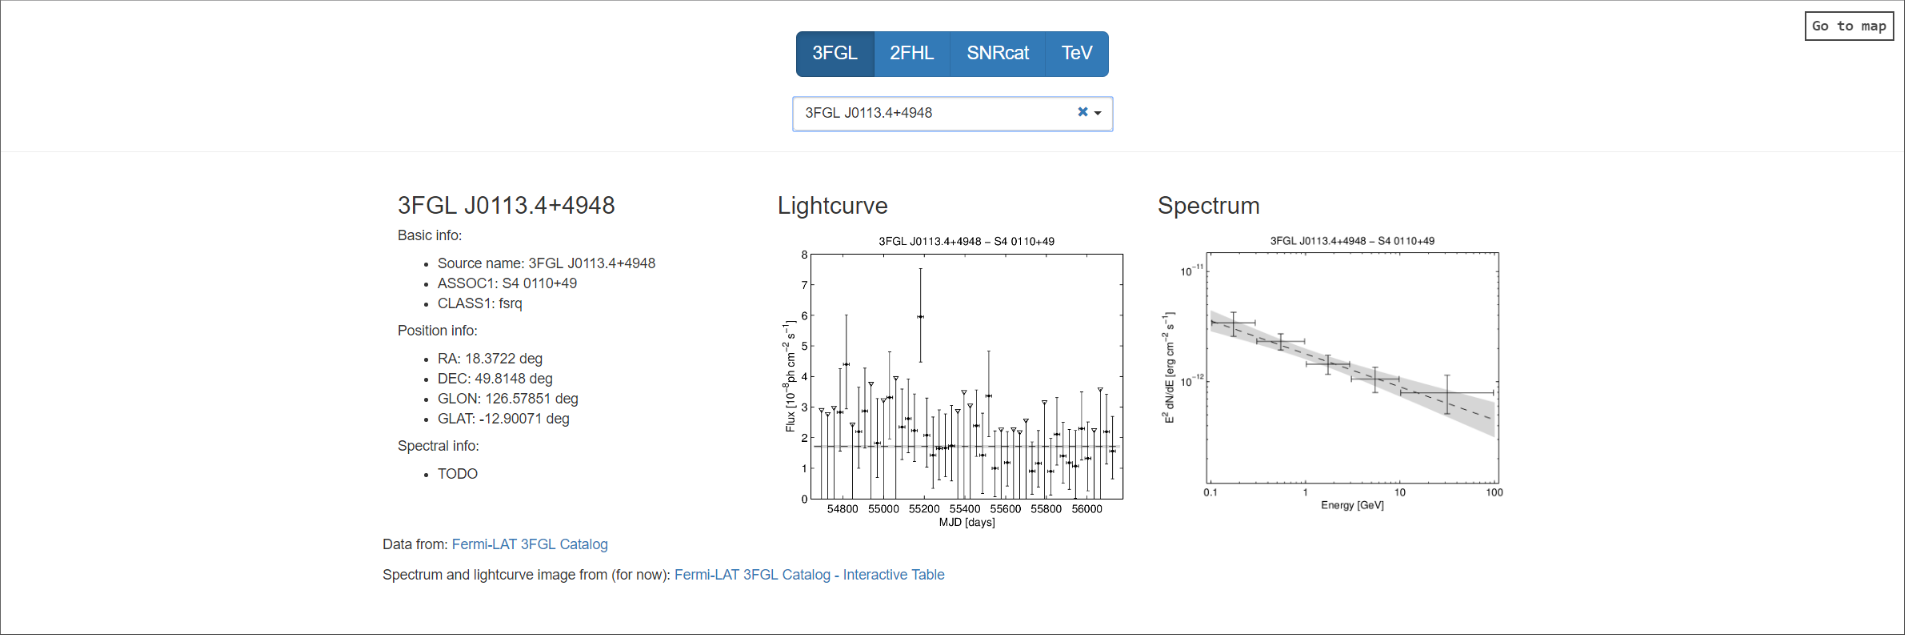
\includegraphics[width=\textwidth]{figures/catview_wide}}
  \caption{Catalog View.}
\end{figure}

\section{Data}

% \cite{2015AnA...578A.114F} HIPS

\begin{enumerate}
\item Survey images

  \begin{itemize}

  \item Default: Fermi color image. Mention other survey options

  \item HiPS file format and HEALPix projection for the map

  \item Our images came from CDS' HiPS database of 300+ images

  \end{itemize}
  
(Image of different surveys on the Aladin Map)
(Table of multi-wavelength surveys on our site)

\item Catalog images

  \begin{itemize}

  \item Fermi-LAT - 3FGL and 2FHL

  \item SNRcat

  \item GeTeV Catalogue

  \end{itemize}
\end{enumerate}

(Table of number of sources per catalog (and maybe also number of sources in each class?))

\section{Implementation}

% \begin{itemize}
% \item Gammapy, Astropy used to generate catalog data (and map data)
% \item Data consumed with JS and HTML
% \item Website architecture built with Angular 2 as a single-page app
% \item Sphere interface and maps overlay by Aladin Lite tool
% \end{itemize}


Scientific Python packages Astropy and Gammapy \cite{gammapy} were used to prepare and generate all of the catalog and source data on gamma-sky.net. The data is consumed with the JavaScript and HTML frontend. The website's architecture was organized using Angular 2, a modern web application framework for JavaScript. Using Angular 2 has allowed us to compile gamma-sky.net into a single-page application. The sphere interface and visualization was implemented using the Aladin Lite tool \cite{aladin-lite} developed at CDS.

TODO: Explain/mention Gammapy in more detail?

\section{Status and Outlook}


Our website is a new project, having been deployed very recently at \url{http://gamma-sky.net} in early June 2016. The website is being hosted by GitHub Pages. The current content of \gammasky is simply a starting point; we have plans to greatly expand on our catalog and image data. Such data includes additional image surveys from CDS' HiPS database, as well as source and image data from upcoming surveys upon their public release. We additionally strive to enhance the user interface of \gammasky through additional features, including new source groupings by classification and position, deeper communication between the Map View and Catalog View, and more intricate data panels for the Catalog View. We will continue to point directly to Gammapy scripts for any further analysis and keep server-heavy tools off our website.

\section{Acknowledgements}

TODO


% References

\nocite{*}
\bibliographystyle{aipnum-cp}
\bibliography{gammaskynet-gamma2016}

\end{document}
